\documentclass{article}
\usepackage[letterpaper,top=2cm,bottom=2cm,left=2cm,right=2cm,marginparwidth=1.75cm]{geometry}
\usepackage[utf8]{inputenc}
\usepackage{graphicx}
\usepackage{caption}
\usepackage{amsmath}

\title{Rapport de Projet NNL\\ Facial recognition: the mask/no mask case}
\author{Hugo Bulzomi, Khaoula Bouhlal}
\date{January 2022}

\begin{document}

\maketitle

\section{Description du projet et de ses objectifs}
Le but de ce projet est de créer un modèle de réseau de neurones capable de discerner les photos d'humains portant un masque (médical) ou non. Nous voulons donc un réseau capable de prendre en entrée une photo de visage humain, et donner en sortie la classe d'appartenance de cette entrée.\\
En addition au modèle de classification pur, nous avons aussi entraîné un second modèle servant uniquement à extraire les visages humains depuis des photos. Le but étant à la fin, de classifier des photos sans aucune intervention humaine. \\
Pour ce faire, nous détaillerons ici les différentes étapes de création de ces modèles : depuis la récolte et le traitements des données utilisées, jusqu'aux tests. Nous prendrons soin de détailler les différentes expérimentations qui nous ont permises d'aboutir aux modèles finaux. Tous les scripts pour reproduire les figures présentées sont trouvables dans le dossier "src/scripts\_for\_report\_figures" de notre projet.

\section{Données employées et leur traitement}
\subsection{Récolte des données}
Conformément au sujet du projet, nous avons tout d'abord récolté un ensemble de photos de personnes de notre entourage. Ces photos incluent donc des visages masqués, et non masqués sous différents angles. Les masques visibles sur ces images sont de natures et de couleurs variées, mais la plupart correspondent au modèle standard de masque chirurgical le plus commun.\\\\

A l'issue de cette récolte de photos, nous avons ainsi rassemblé 84 photos non traitées. Trois exemples de photo non traitées sont visibles sur la figure 1.

\begin{figure}[h]
\centering
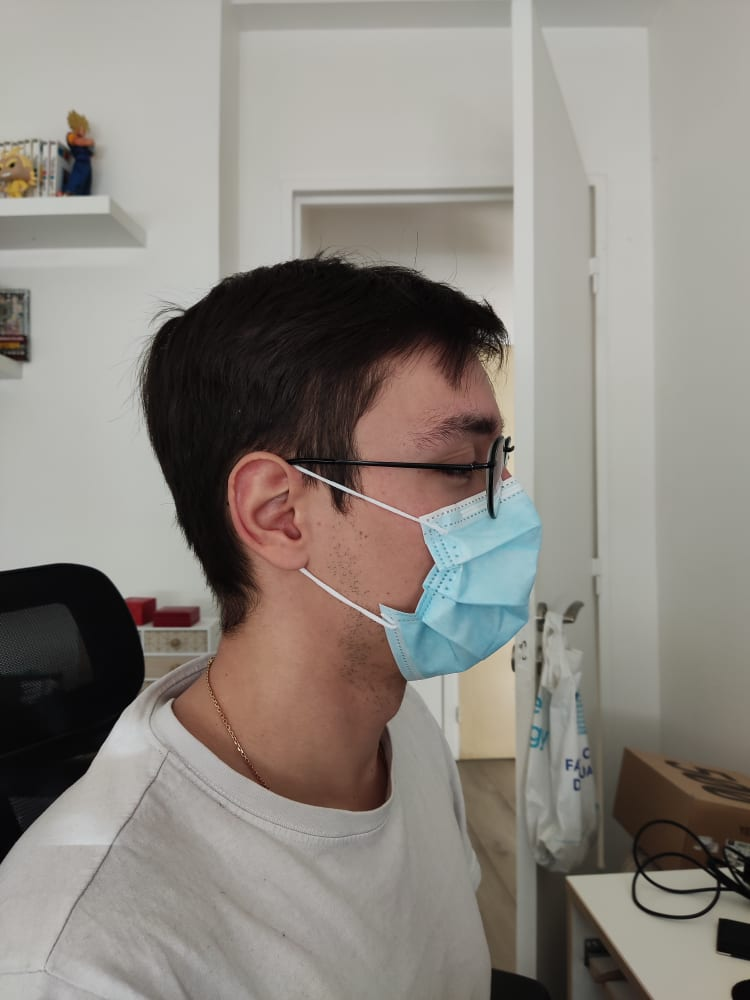
\includegraphics[width=0.25\textwidth]{non_traite1.jpg}
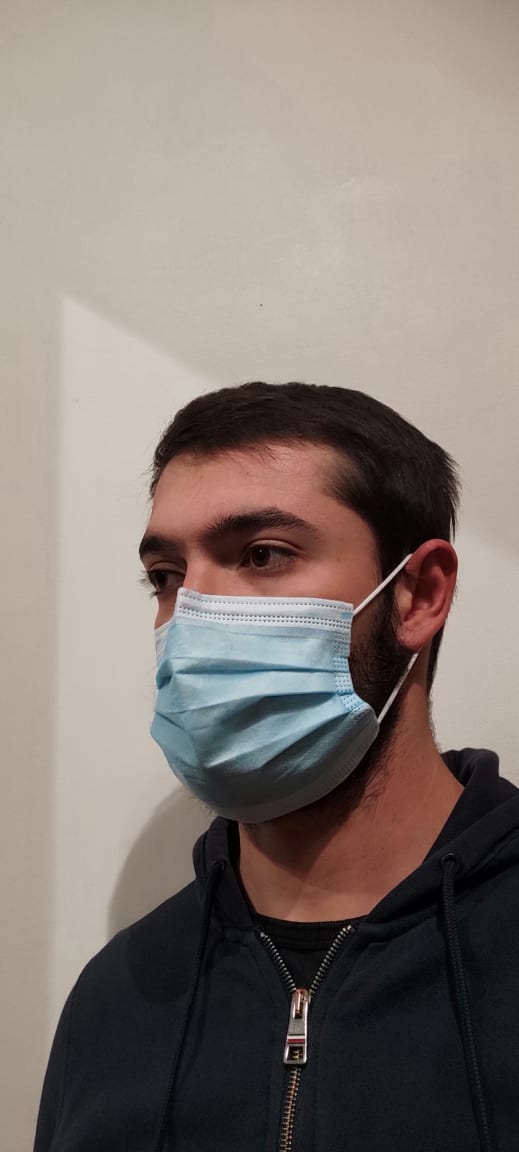
\includegraphics[width=0.15\textwidth]{non_traite3.jpg}
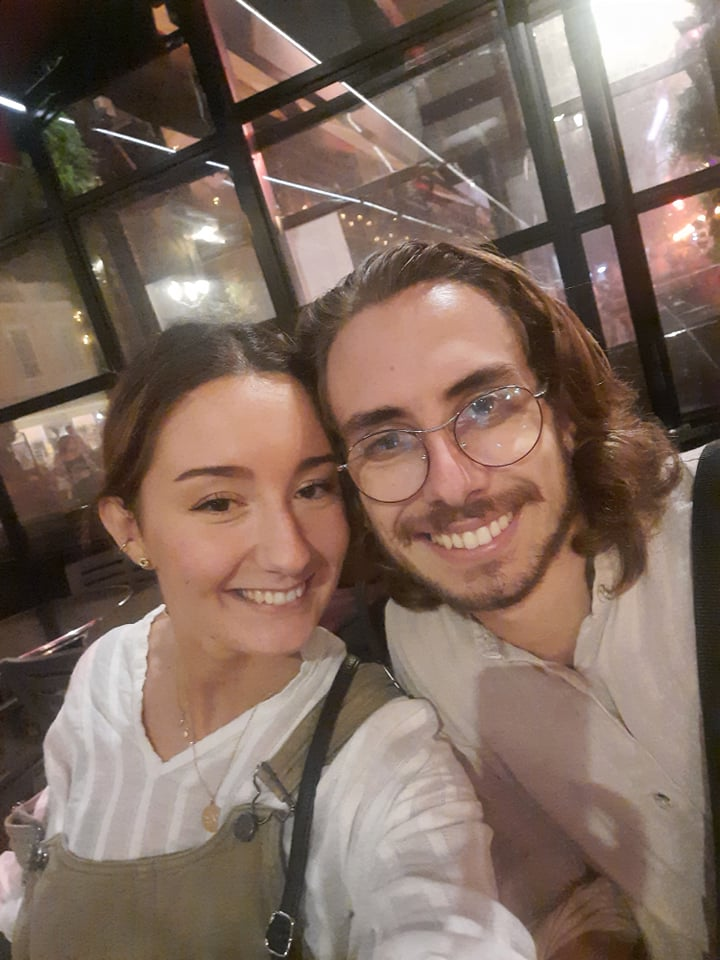
\includegraphics[width=0.25\textwidth]{non_traite2.jpg}
\caption{\label{fig:Input}Trois exemples de photo originales non traitées. On constate que les visages ne sont pas particulièrement bien détourés ou en gros plan. L'angle de vue peut varier et certaines photos contiennent plusieurs visages.}
\end{figure}



\subsection{Traitement des données}
Les images obtenues précédemment ne sont pas encore directement utilisables pour entraîner un modèle de réseau de neurones. En effet, nous devons encore délimiter les contours rectangles de chaque visage sur ces photos, et les annoter avec des labels indiquant si la personne en question porte un masque ou pas.\\\\

Pour ce faire, nous avons utilisé l'annotateur produit durant la première partie de ce projet. Nous avons passé en revue chaque photo que nous avons récoltée, et appliqué le traitement suivant:
\begin{itemize}
  \item Ouvrir l'image dans l'annotateur.
  \item Délimiter un rectangle autour de chaque visage présent sur l'image.
  \item Après la création de chaque rectangle, l'annotateur demande d'entrer un label pour ce rectangle. On choisi alors entre les catégories "mask" ou "no\_mask".
  \item Une fois tous les visages annotés, on enregistre les annotations. L'annotateur sauvegarde alors chaque rectangle créé comme une image à part entière don le nom suit le standard: myimage-bb-XxY-W-H.png où myimage est le nom de l'image originale, X et Y les c oordonnées du rectangle, et W et H ses dimensions.
  \item L'annotateur redimensionne les images ainsi créées afin d'obtenir des images carrées de tailles $128\times128$.
  \item Finalement, l'annotateur enregistre la nouvelle image créée dans un dossier différent en fonction de son label.\\
\end{itemize}

A la fin de ce procédé, nous obtenons ainsi une image carrée de taille $128\times128$ pour chaque visage présent sur les photos originales, accompagnée de sa classe d'appartenance (un dossier différent pour chaque classe). La figure 2 montre les images obtenues pour les photos de la figure 1 après cette phase d'annotation.
\begin{figure}[h]
\centering
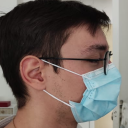
\includegraphics[width=0.15\textwidth]{annotated2.png}
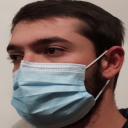
\includegraphics[width=0.15\textwidth]{annotated1.png}
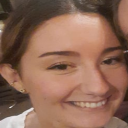
\includegraphics[width=0.15\textwidth]{annotated4.png}
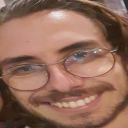
\includegraphics[width=0.15\textwidth]{annotated3.png}
\caption{\label{fig:Input}Les visages de la figure 1 ont été annotés et enregistrés dans deux dossier différent en fonction de leur catégorie.\\}
\end{figure}

Nous obtenons ainsi exactement 100 visages parfaitement cadrés. Parmi eux, exactement 50 portent un masque, et 50 autres n'en portent pas. Les images ainsi créées sont donc chargées comme des tableaux de forme $(128\times128\times4)$. Nous avons donc des images de 128 pixels par 128 pixels avec 4 canaux de couleur (rouge, bleu, vert et alpha). Ces canaux de couleurs contiennent des valeurs entre 0 et 255.\\
Avant l'entraînement nous divisons chaque canal de couleur par 255 afin d'obtenir des valeurs entre 0.0 et 1.0, et nous enlevons le canal alpha. Ainsi, le dataset final contient des images de forme $(128\times128\times3)$. Pour finir, $70\%$ des images sont listées pour entrainer le modèle, et les $30\%$ restantes seront utilisées pour le tester. Les images sont mélangées avant chaque entraînement afin de ne pas obtenir les mêmes groupes à chaque fois.

\section{Méthode et expérimentations}
\subsection{Méthode d'entraînement et de test}
Après avoir traité les photos de base et avoir obtenu un dataset comme expliqué précédemment, il était temps de s'intéresser au modèle de classification en lui même.\\\\

Il peut être difficile de choisir une architecture et des paramètre pour un modèle puisqu'il n'existe pas de règles formelles pour cela. Nous avons donc testé différentes architecture et trouvé expérimentalement celle qui nous convenait le mieux. Notre méthode expérimentale est la suivante:
\begin{itemize}
  \item Nous chargeons les images traitées et formons nos groupes d'entraînement et de test.
  \item Nous définissons ensuite une liste de modèles à tester à l'aide de la librairie Tensorflow.
  \item Nous entraînons chaque modèle pour un certain nombre d'epochs.
  \item Finalement nous notons l'accuracy, sur le dataset d'entraînement et de test, et la matrice de confusion sur ce dernier. Nous réitérons les deux derniers points plusieurs fois afin d'obtenir une accuracy moyenne sur notre dataset de test et d'entraînement.
  \item Quand tous les modèles ont été testés plusieurs fois, nous analysons les résultats pour trouver quel modèle nous permet d'obtenir les meilleurs résultats.\\
\end{itemize}

Il est à noter que pendant cette première partie expérimentale, nous ne prenons en compte que l'accuracy pendant la phase d'entraînement et de test. Puisque nous avons exactement 50 visages masqués et 50 visages sans masque, un modèle non-entraîné a une accuracy d'environ 0.5. De plus, nous ne testons ici que le modèle de classification pur. Le modèle servant à prédire les cadres des visages sur une photo sera traité plus tard.\\
Dans l'ordre, nous avons tout d'abord voulu trouver combien de couches de convolution étaient nécessaires et avec combien de filtres. Puis, combien de couches de dropout. Et enfin le ratio de dropout approprié.\\

\subsection{Le nombre de couches de convolution}
Comme énoncé précédemment, notre première batterie de test a porté sur le nombre de couche de convolution et le nombre de filtre pour ces dernières. Afin de réduire le nombre de modèle à tester, nous nous imposons de respecter certaines lignes directives :
\begin{itemize}
  \item Le nombre de filtres de convolution va croissant avec la profondeur du modèle.
  \item Une couche de convolution est suivie d'une couche de maxpooling.\\
\end{itemize}

En respectant ces deux règles, nous avons testé 5 architectures différentes comprenant respectivement une, deux, trois, quatre et cinq couches de convolution. Dans chacun de ces modèles, le nombre de filtre est multiplié par 2 à chaque nouvelle couche de convolution. La figure 3 montre le résumé de ces modèles de base.
\begin{figure}[h]
\centering
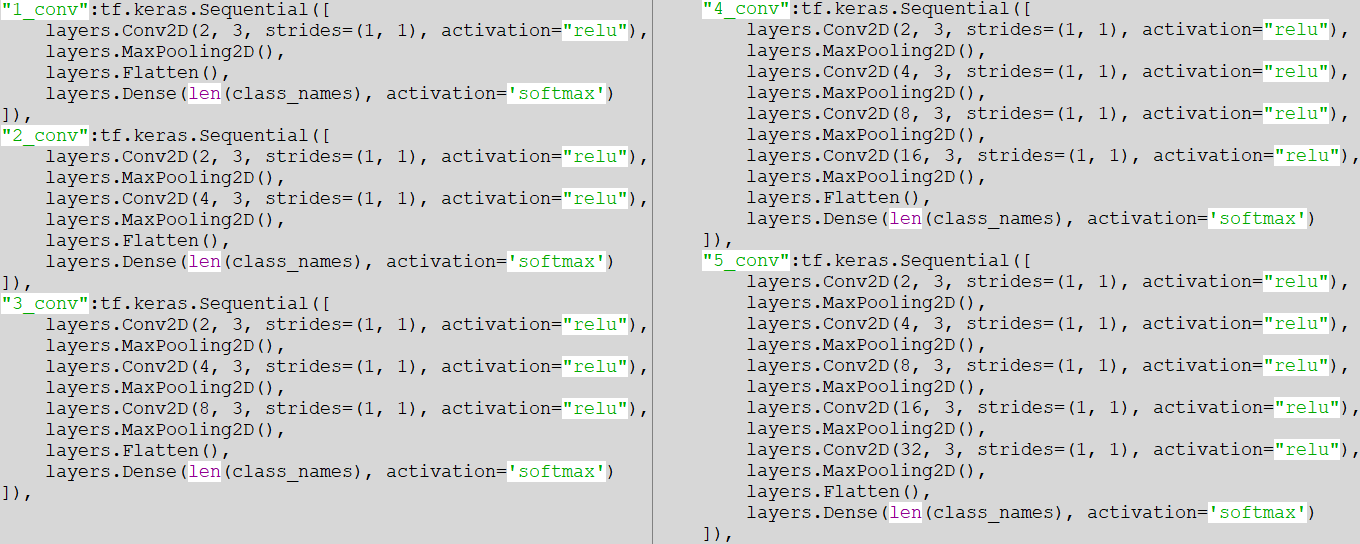
\includegraphics[width=1.0\textwidth]{base_models.png}
\caption{\label{fig:Input}La définition des 5 modèles de base sur lesquels nous nous basons. \\}
\end{figure}

La figure 3 montre que le nombre de filtre va croissant dans chaque convolution. L'activation de type "relu" pour les convolutions a été choisis car conseillé par le tutoriel inclut dans le sujet du projet. La couche de type flatten permet simplement d'éliminer à la fin les dimensions en plus que nous avons du fait de garder les couleurs des images. L'activation de la couche de sortie est de type "softmax" afin de quantifier la confiance en une prédiction comme une probabilité.\\

Basé sur ces 5 modèles de base, nous avons aussi créé 5 variantes de ces derniers en multipliant leur nombre de filtre par 2, puis encore 5 autres en multipliant leur nombre de filtre par 4.\\
Ainsi, nous avons testé en tout 15 modèles différents pour trouver le nombre de couche de convolution et de filtre approprié. Ces 15 modèles sont trouvables dans le script "src/scripts\_for\_report\_figures/figure4.py" de notre projet.\\La figure 4 montre les résultats obtenus.\\
\begin{figure}[h]
\centering
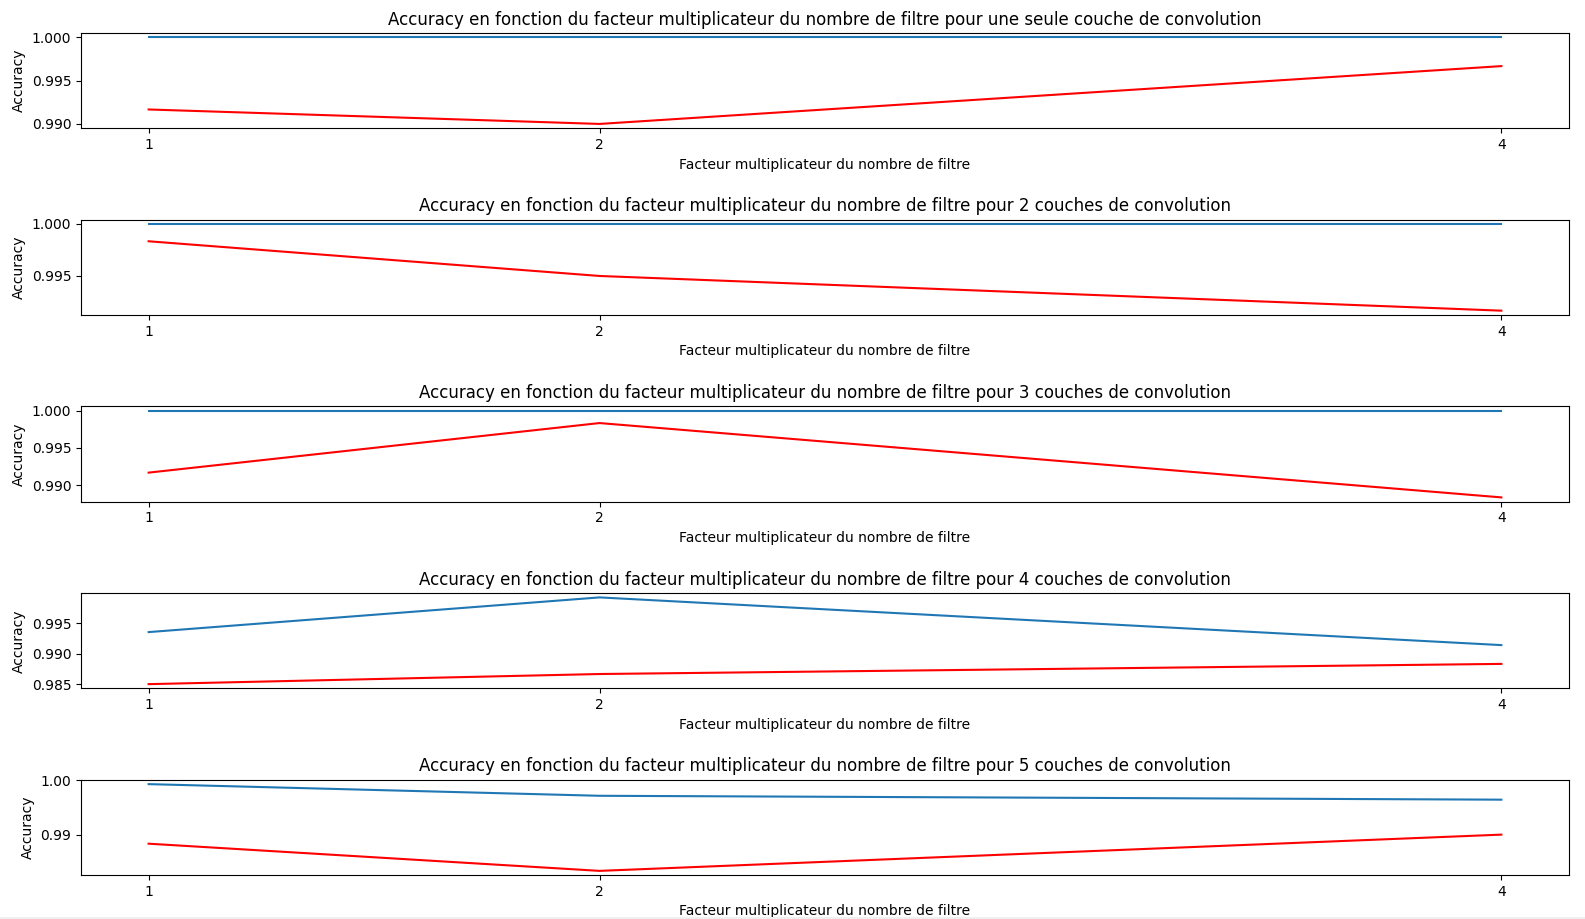
\includegraphics[width=1.0\textwidth]{results_convo_test.png}
\caption{\label{fig:Input}On observe ici l'accuracy pendant l'entrainement (en bleu) et pendant le test (en rouge). Chaque graphe montre l'évolution de ces métriques pour chaque modèle (1, 2, 3, 4, ou  5 couches de convolution), en fonction du facteur mutiplicatif du nombre de filtre. Ces données sont les valeurs moyennes obtenues après 20 itérations d'entraînement sur 10 epochs pour chaque modèle.\\}
\end{figure}

La figure 4 nous permet ainsi de constater que les résultats sont de façon générale très bons. On constate néanmoins un ovefitting consistant puisque l'accuracy pendant l'entrainement est toujours plus haute que celle durant le test. \\
A ce stade, nous pourrions choisir n'importe lequel de ces modèles. Nos graphes montrent néanmoins que le modèle avec 3 couches de convolution et un facteur multiplicatif de 2 pour le nombre de filtre semble légèrement meilleur que les autres. Nous garderons donc cette architecture pour les tests suivants.

\subsection{Le nombre de couches de dropout}
Afin d'essayer de diminuer l'overfitting de notre modèle, nous avons testé ses performances en ajoutant une, deux et trois couches de dropout. La figure 5 montre les trois modèles que nous avons ainsi testés.\\\\\\
\begin{figure}[h]
\centering
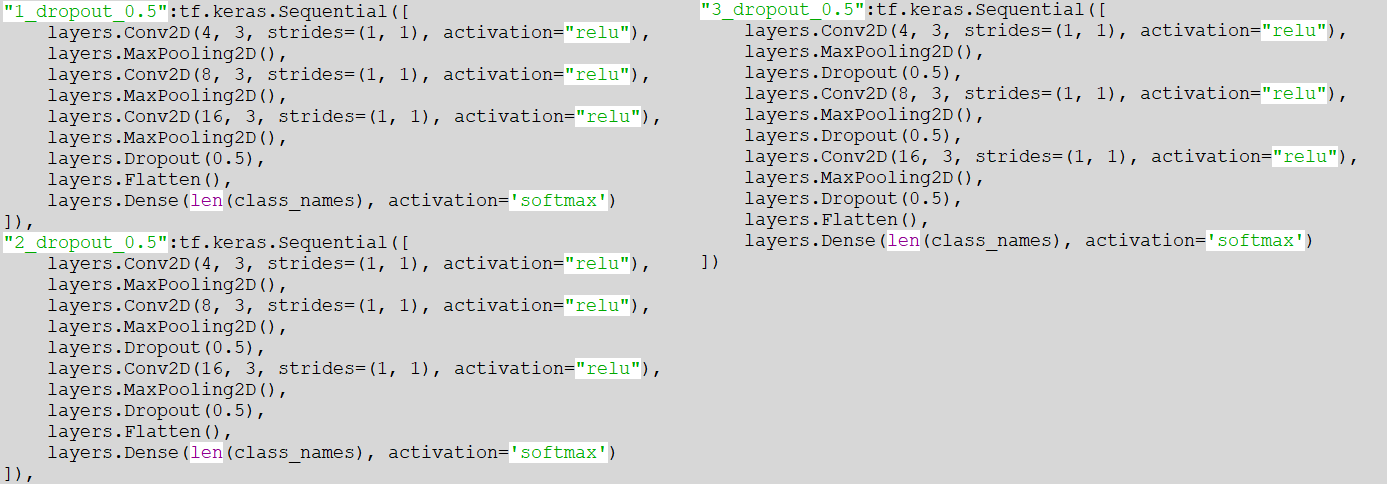
\includegraphics[width=0.9\textwidth]{dropout_models.png}
\caption{\label{fig:Input}La définition des 3 modèles avec dropout basé sur l'architecture à 3 couches de convolution qui a montré les meilleurs résultats précédemment.\\}
\end{figure}

Le ratio de dropout est dans un premier temps réglé à 0.5. C'est en effet une valeur assez populaire et standard pour ce genre de couche. La figure 6 montre maintenant les résultats obtenus en faisant varier le nombre de couche de dropout.
\begin{figure}[h]
\centering
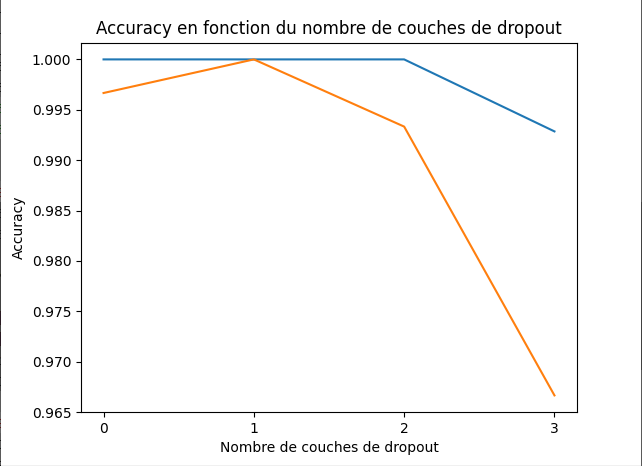
\includegraphics[width=0.5\textwidth]{dropout_var.png}
\caption{\label{fig:Input}On observe ici l'accuracy pendant l'entrainement (en bleu) et pendant le test (en orange), en fonction du nombre de couches de dropout. Ces valeurs sont les moyennes obtenues après 20 itérations de 20 epochs d'entraînement pour chaque modèle.}
\end{figure}

La figure 6 permet ainsi de constater que n'avoir qu'une couche de dropout semble donner les meilleurs résultats. De cette façon on augmente notre accuracy pendant le test et réduisons donc l'overfitting de notre modèle.\\

Il ne nous reste à présent qu'à tester différentes valeurs de ratio de dropout, comme le montre la figure 7.\\\\\\\\\\\\\\\\\\

\begin{figure}[ht]
\centering
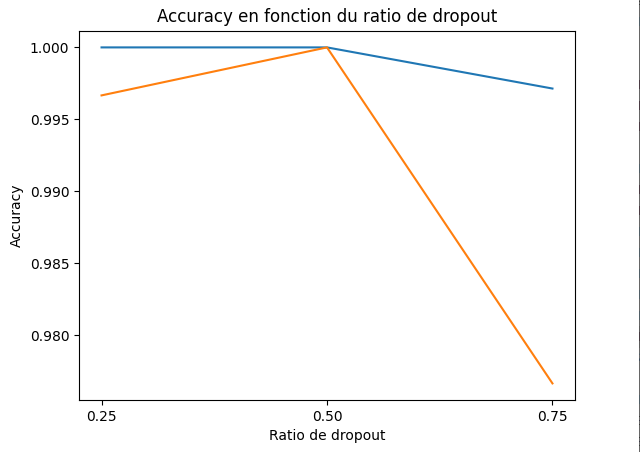
\includegraphics[width=0.5\textwidth]{dropout_ratio.png}
\caption{\label{fig:Input}On observe ici l'accuracy pendant l'entrainement (en bleu) et pendant le test (en orange), en fonction du nombre du ratio de dropout. Ces valeurs sont les moyennes obtenues après 20 itérations de 20 epochs d'entraînement pour chaque modèle.}
\end{figure}

En conclusion de cette partie d'expérimentation, nous avons trouvé qu'un réseau comprenant trois convolutions et une couche de dropout était approprié pour notre projet. les spécifications exactes de notre classificateur sont ainsi décrites dans la figure 8.
\begin{figure}[h]
\centering
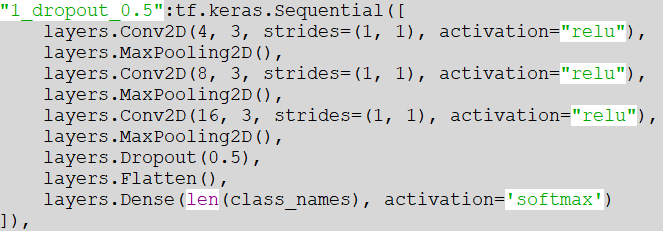
\includegraphics[width=0.6\textwidth]{model_specs_final.png}
\caption{\label{fig:Input}Spécification du modèle retenu après expérimentation.}
\end{figure}

\subsection{Second modèle pour l'extraction des visages depuis des photos }
Étant satisfait de notre classificateur, nous voulions à présent être capable d'extraire les visages depuis des photos de façon automatique. L'idée étant de montrer que notre projet est applicable à des données "réelles", c'est à dire à des photos non traitées.\\
Nous nous somme largement basé sur l'architecture du modèle de classification, modifiant uniquement la taille de l'entrée, la taille de la sortie, et le mode d'activation des neurones sur la couche de sortie. La figure 9 montre la définition du modèle.\\\\\\\\\\\\\\\\\\\\\\
\begin{figure}[hpt]
\centering
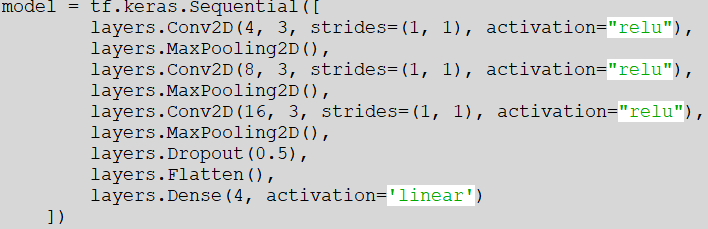
\includegraphics[width=0.5\textwidth]{model_face_extrator.png}
\caption{\label{fig:Input}Spécification du modèle servant à reconnaître les limites du cadre délimitant un visage humain sur une photo.\\}
\end{figure}

Par soucis de simplicité (et car nous n'étions pas sûr que la création d'un tel modèle était attendue), ce modèle ne pourra reconnaître qu'un visage par photo. Le principe derrière son entraînement est simple:
\begin{itemize}
  \item Nous chargeons les photos originales, non-annotées.
  \item Nous chargeons les noms uniquement des images de visages créés à la main pour chaque photo originale.
  \item On peut ainsi associer à chaque photo originale, les coordonnées et dimensions du cadre du visage qui s'y trouve. Ces coordonnées sont trouvables car l'annotateur les a sauvegardés dans le titre de l'image sauvegardée après annotation (voir partie 2.2).
  \item Les photos avec plus d'un visage présent ne sont pas prises en compte. Nous pourrions parfaitement entraîner notre modèle à reconnaître plus d'un visage par photo, mais notre collection ne contient que très peu d'images avec plusieurs visages. Probablement trop peu pour entraîner notre modèle dessus.
  \item Les photos originales sont dimensionnées pour être de taille $(300\times300)$.
  \item Enfin, nous attendons de notre modèle, une sortie de taille 4 où les deux premiers nombres correspondent aux coordonnées haut-gauche du cadre du visage sur la photo, et le deux derniers la largeur et hauteur de celui-ci. \\
  
  Nous avons ainsi entraîné ce second modèle pour 30 epochs, à l'image de notre modèle de classification. Les résultats pour ces deux modèles vont maintenant être décrit dans la prochaine section.
\end{itemize}





\section{Résultats du modèle de prédiction final}
L'architecture du modèle ayant été expérimentalement définie, il ne nous reste alors plus qu'à la tester en pratique. Dans cette partie nous allons tout d'abord montrer les résultats obtenus pour la classification pure de visage avec notre premier modèle. Nous verrons rapidement ensuite les performances de notre second modèle devant reconnaître le cadre d'un visage présent sur une photo non traitée. Enfin, nous ferons travailler ces deux modèles de concert afin de classifier les visages présents sur nos photos originales, non traitées (en ne prenant en compte que les photos contenant un seul visage).

\subsection{Résultats sur notre dataset de visages déjà extraits à la main}
L'architecture du modèle ayant été choisie expérimentalement, nous pouvons maintenant analyser ses résultats. La figure 10 montre l'évolution de différentes métriques vues en cour en faisant varier le temps d'entraînement. Il est à noter que les métriques présentées sont calculées directement sur la matrice de confusion produite pendant la phase de test. Le modèle produisant des probabilités de classification en sorties, la classification finale se fait simplement en choisissant la classe ayant la plus haute probabilité selon notre modèle.\\\\\\\\\\\\\\
\begin{figure}[h]
\centering
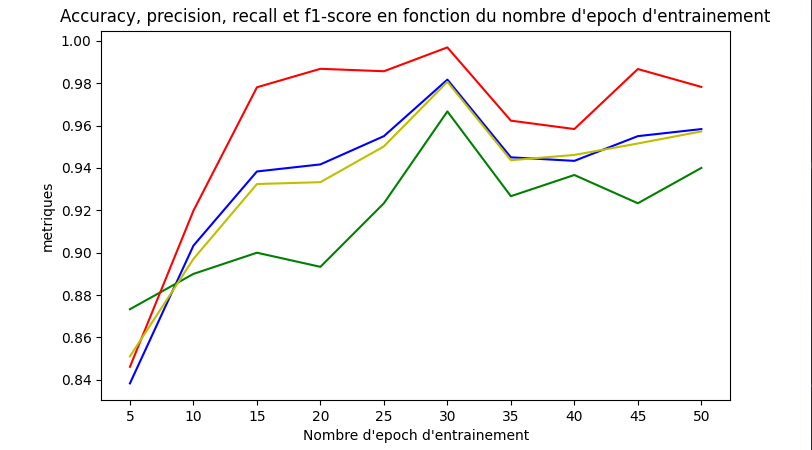
\includegraphics[width=0.8\textwidth]{metrics_epoch.png}
\caption{\label{fig:Input}Variation de l'accuracy (bleu), de la précision (verte), du recall (rouge) et du F1-score (jaune) en fonction du nombre d'epoch d'entraînement. Les données présentées sont des moyennes obtenues sur 20 itérations où le modèle est entraîné sur $70\%$ du dataset et testé sur $30\%$. Les métriques ne sont mesurées que sur le dataset de test.}
\end{figure}

Tout d'abord, nous pouvons observer que 30 epochs semblent suffisantes pour obtenir d'excellents résultats. Dans un second temps, le recall est plus élevé que la précision et ce, de façon consistante. Ce résultat semble indiquer que notre modèle à tendance à produire plus de faux positifs que de faux négatifs : ce dernier a plus de facilité à reconnaître si une personne porte un masque, qu'à reconnaître si cette personne n'en porte pas. Le F1-score, quant à lui, suit le recall de près.\\
En addition à la figure 10, la table 1 montre une matrice de confusion produite sur l'intégralité de notre dataset. \\

\begin{tabular}{ |p{2cm}||p{2cm}|p{2cm}| }
 \hline
   & Nomask &Mask \\
 \hline
  Nomask & 50 & 0 \\
 Mask & 0 & 50 \\
 \hline
\end{tabular}
\captionof{table}{Matrice de confusion obtenue sur notre dataset entier d'images de visages. Le modèle testé a été entraîné pour 30 epochs sur $70\%$ du dataset et testé sur son intégralité.\\}

On constate alors une classification parfaite. Comme le montre le graphe de la figure 10, la matrice de confusion n'est néanmoins pas toujours aussi parfaite. Selon l'initialisation aléatoire de l'entraînement, les résultats peuvent légèrement varier. De façon générale, la classification est néanmoins toujours de qualité et le recall souvent un peu au dessus de la précision. \\

Ces résultats montrent que notre modèle est parfaitement adapté à classifier des visages de personnes masquées ou sans masque. N'étant pas totalement sûr de si ces résultats suffisaient pour conclure ce projet, nous avons aussi voulu tester notre modèle directement sur nos photos originales.

\subsection{Résultats de notre modèle d'extraction de visages}
Comme mentionné plus tôt, notre second modèle est sensé prendre une photo contenant un visage unique en entrée, et donner en sortie les coordonnées et dimensions du cadre contenant ce visage. Après un entraînement de 30 epochs, la figure 11 montre quelques exemples des cadres prédits par ce modèle sur des photos du dataset de test.\\\\\\\\
\begin{figure}[h]
\centering
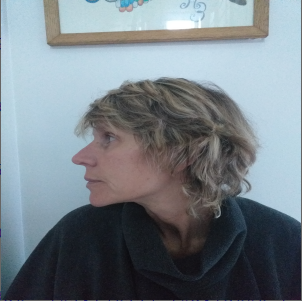
\includegraphics[width=0.3\textwidth]{original_resized5.png}
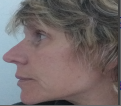
\includegraphics[width=0.15\textwidth]{extracted5.png}
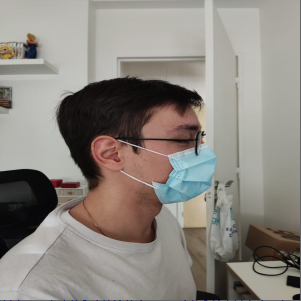
\includegraphics[width=0.3\textwidth]{original_resized4.png}
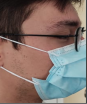
\includegraphics[width=0.15\textwidth]{extracted4.png}
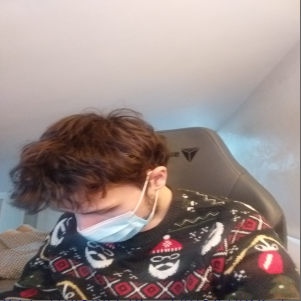
\includegraphics[width=0.3\textwidth]{original_resized3.png}
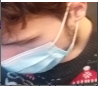
\includegraphics[width=0.15\textwidth]{extracted3.png}
\caption{\label{fig:Input}Trois photos originales, et le visage extrait par notre modèle.\\}
\end{figure}

L'entraînement s'est fait en utilisant la loss function "mean square error". En d'autres termes, l'erreur de prédiction du modèle est mesurée comme la différence moyenne au carrée entre les coordonnées et dimensions prédites pour le cadre, et les dimensions attendues. Après 30 epochs d'entraînement, cette loss est de 7.0 sur le dataset d'entraînement et de 28.1 sur celui de test. Nous avons donc un peu d'overfitting sur ce modèle. Néanmoins, l'unité utilisée pour mesurer cette erreur étant le pixel, une imprécision de 28.1 pixels en moyenne est parfaitement acceptable pour conclure notre projet.

\subsection{Prédicteur final utilisant les deux modèles}
Nous pouvons à présent enfin créer un prédicteur global alliant les deux modèles vus précédemment. La méthode de test va ici consister à charger une photo de base, en extraire le visage grâce à notre modèle d'extraction, puis le faire classifier par notre classificateur. Nous savons déjà que le classificateur a de très bons résultats sur l'ensemble de notre dataset de visages détourés à la main. Nous allons donc ici directement tester le prédicteur constitué de nos deux modèles sur l'ensemble des photos originales ne contenant qu'un seul visage. La table 2 montre ainsi les performances de notre prédicteur final sur l'ensemble de nos photos.\\\\
\begin{tabular}{ |p{2cm}||p{2cm}|p{2cm}| }
 \hline
   & Nomask & Mask \\
 \hline
  Nomask & 27 & 4 \\
 Mask & 0 & 28 \\
 \hline
\end{tabular}
\captionof{table}{Matrice de confusion obtenue pour notre prédicteur alliant nos deux modèles sur la totalité de nos photos originales.\\}
Puisque l'on ne prend en compte ici que les images ne contenant un seul visage, nous avons en tout 59 photos. Nous pouvons calculer les métriques vues précédemment pour cette matrice:\\
$accuracy = 93$ \\   $precision = 0.88$ \\   $recall = 1.0$ \\   $f1-score = 0.93$\\

Le prédicteur global arrive donc en effet à classifier correctement des images non traitées dans la majorité des cas. Les résultats vus ici sont cohérents avec ceux observés dans la figure 10 : le prédicteur semble trop enclin à classifier une personne comme "portant un masque".\\
Pour terminer, comme spécifié dans la consigne, nous avons écrit un dernier script permettant de charger les deux modèles, et de prédire la classe d'une image à l'aide d'une méthode "predict". Cette méthode prend en entrée le chemin d'une image non-annotée, et un mode ("probabilities" ou "categories"). La figure 12 montre deux exemples d'utilisation.\\
\begin{figure}[h]
\centering
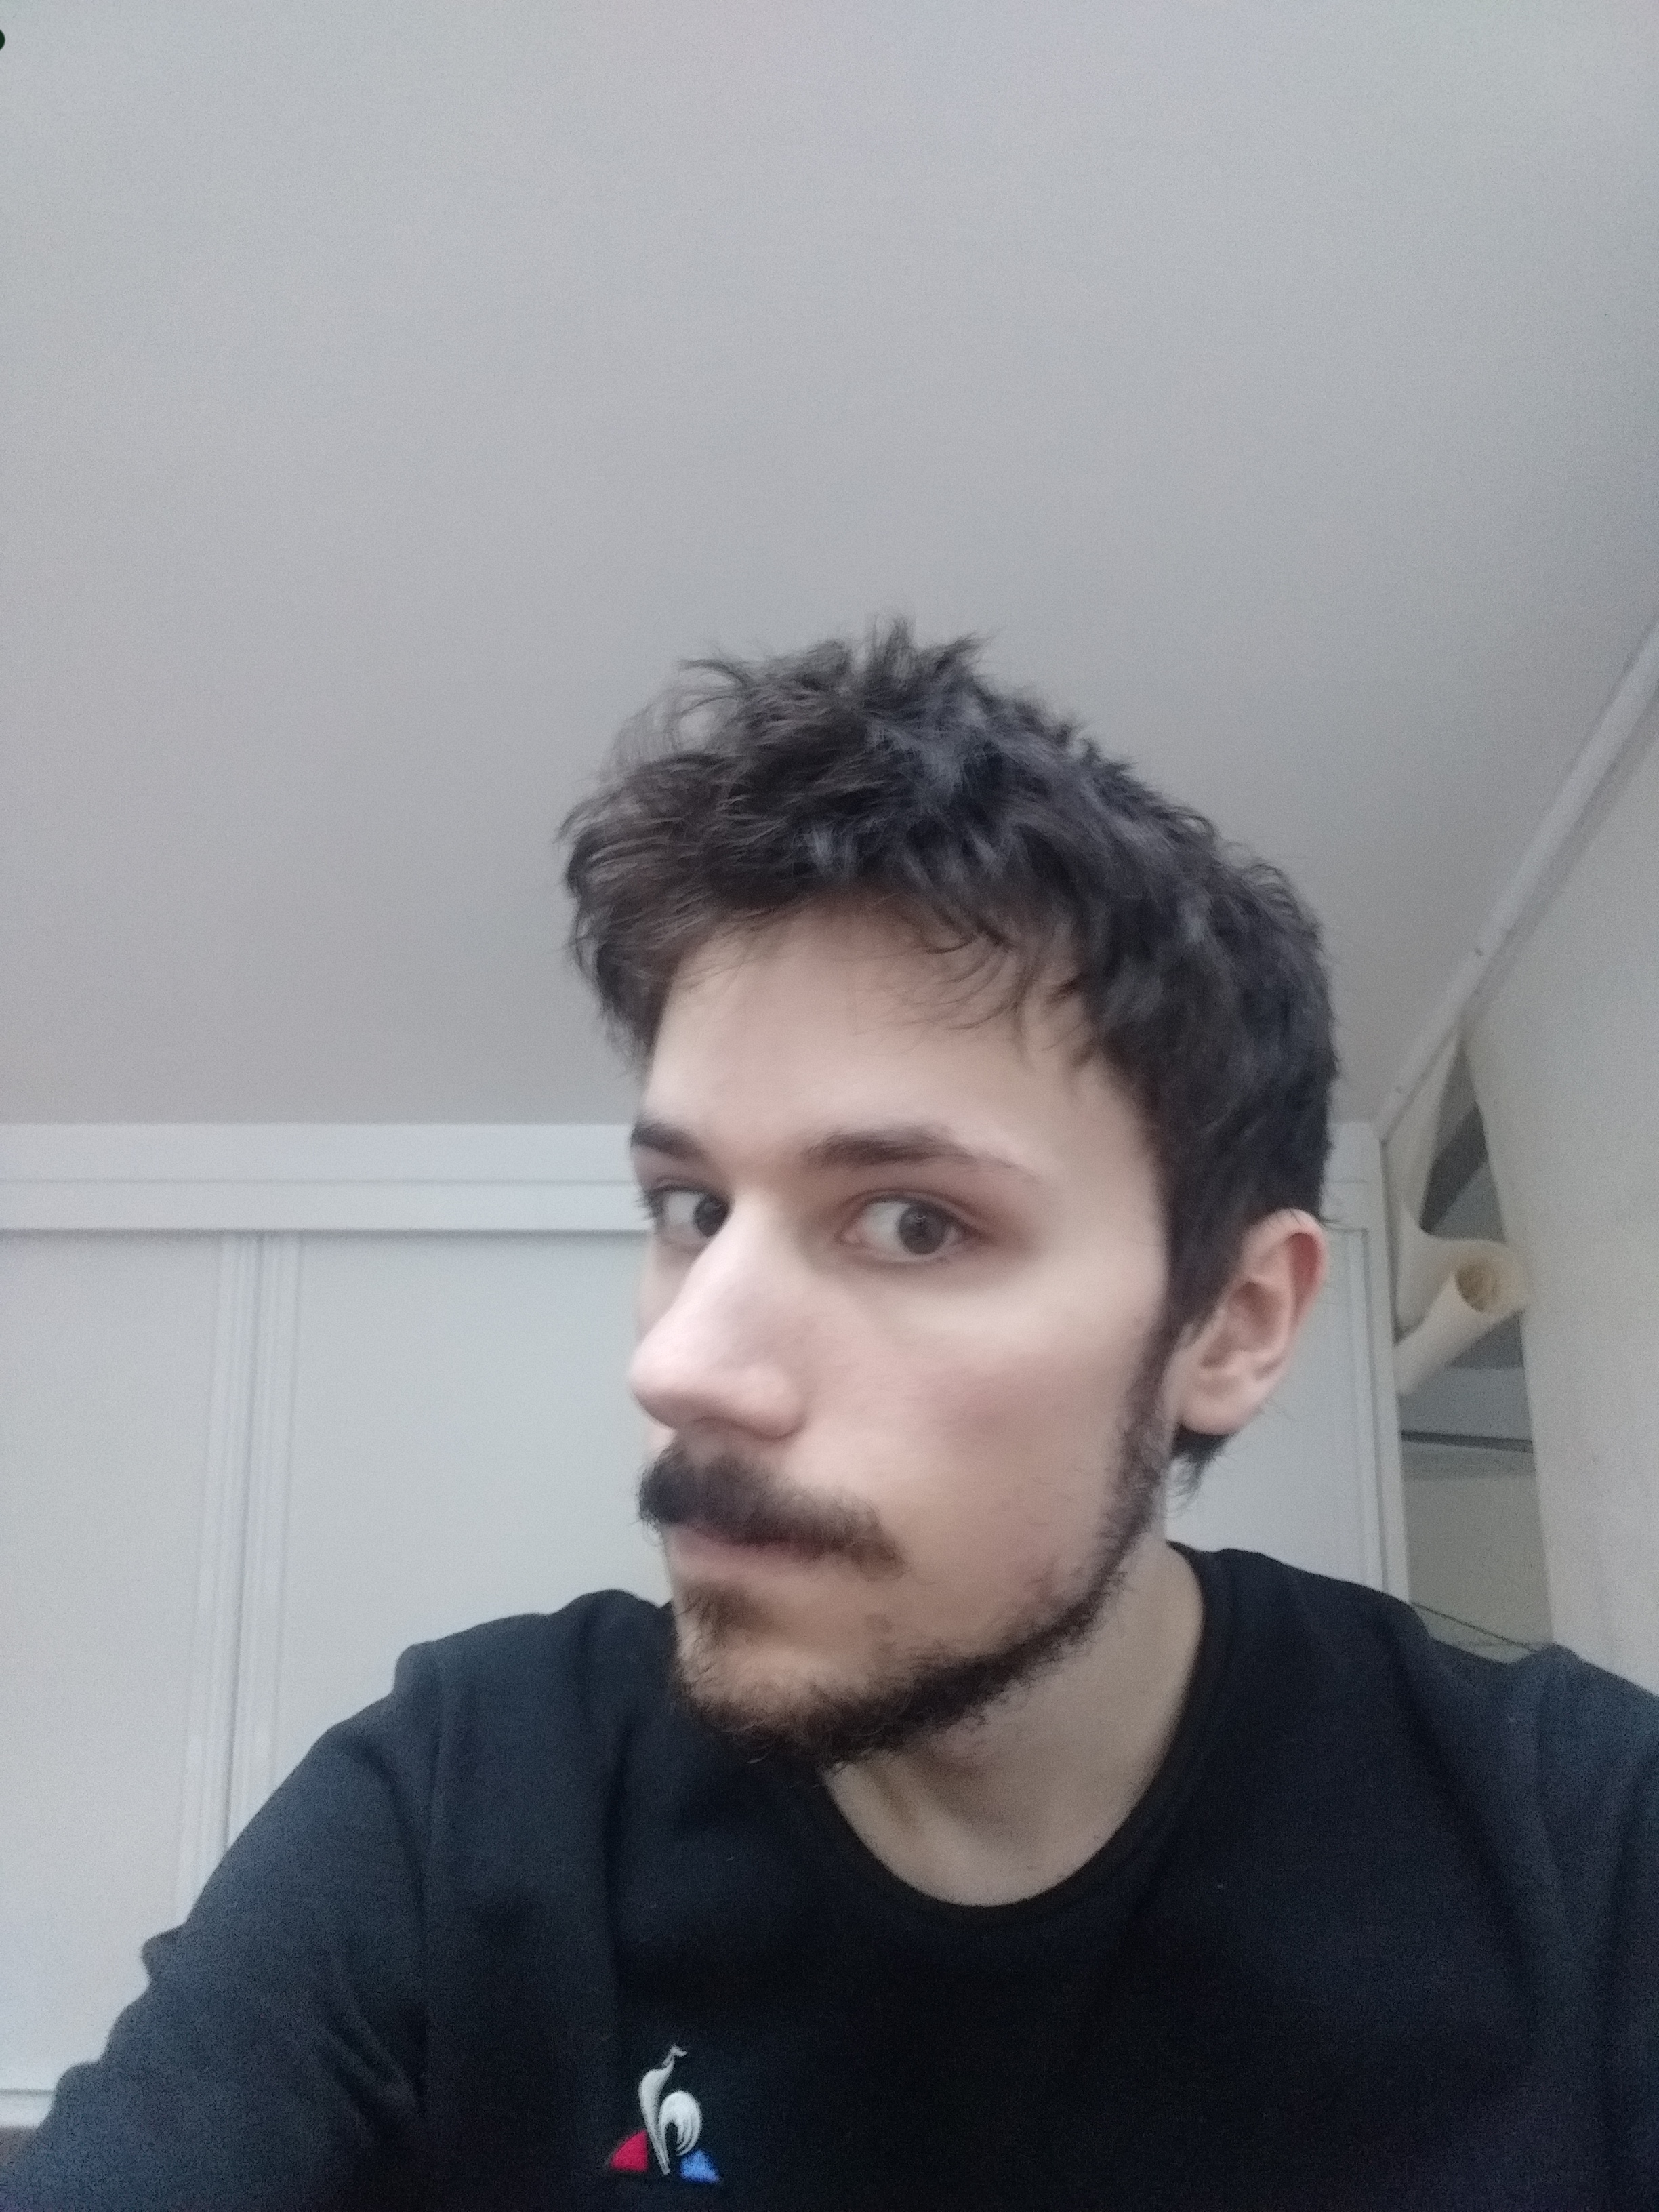
\includegraphics[width=0.2\textwidth]{20220115_150828.jpg}
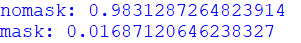
\includegraphics[width=0.25\textwidth]{pred_probabilities.png}
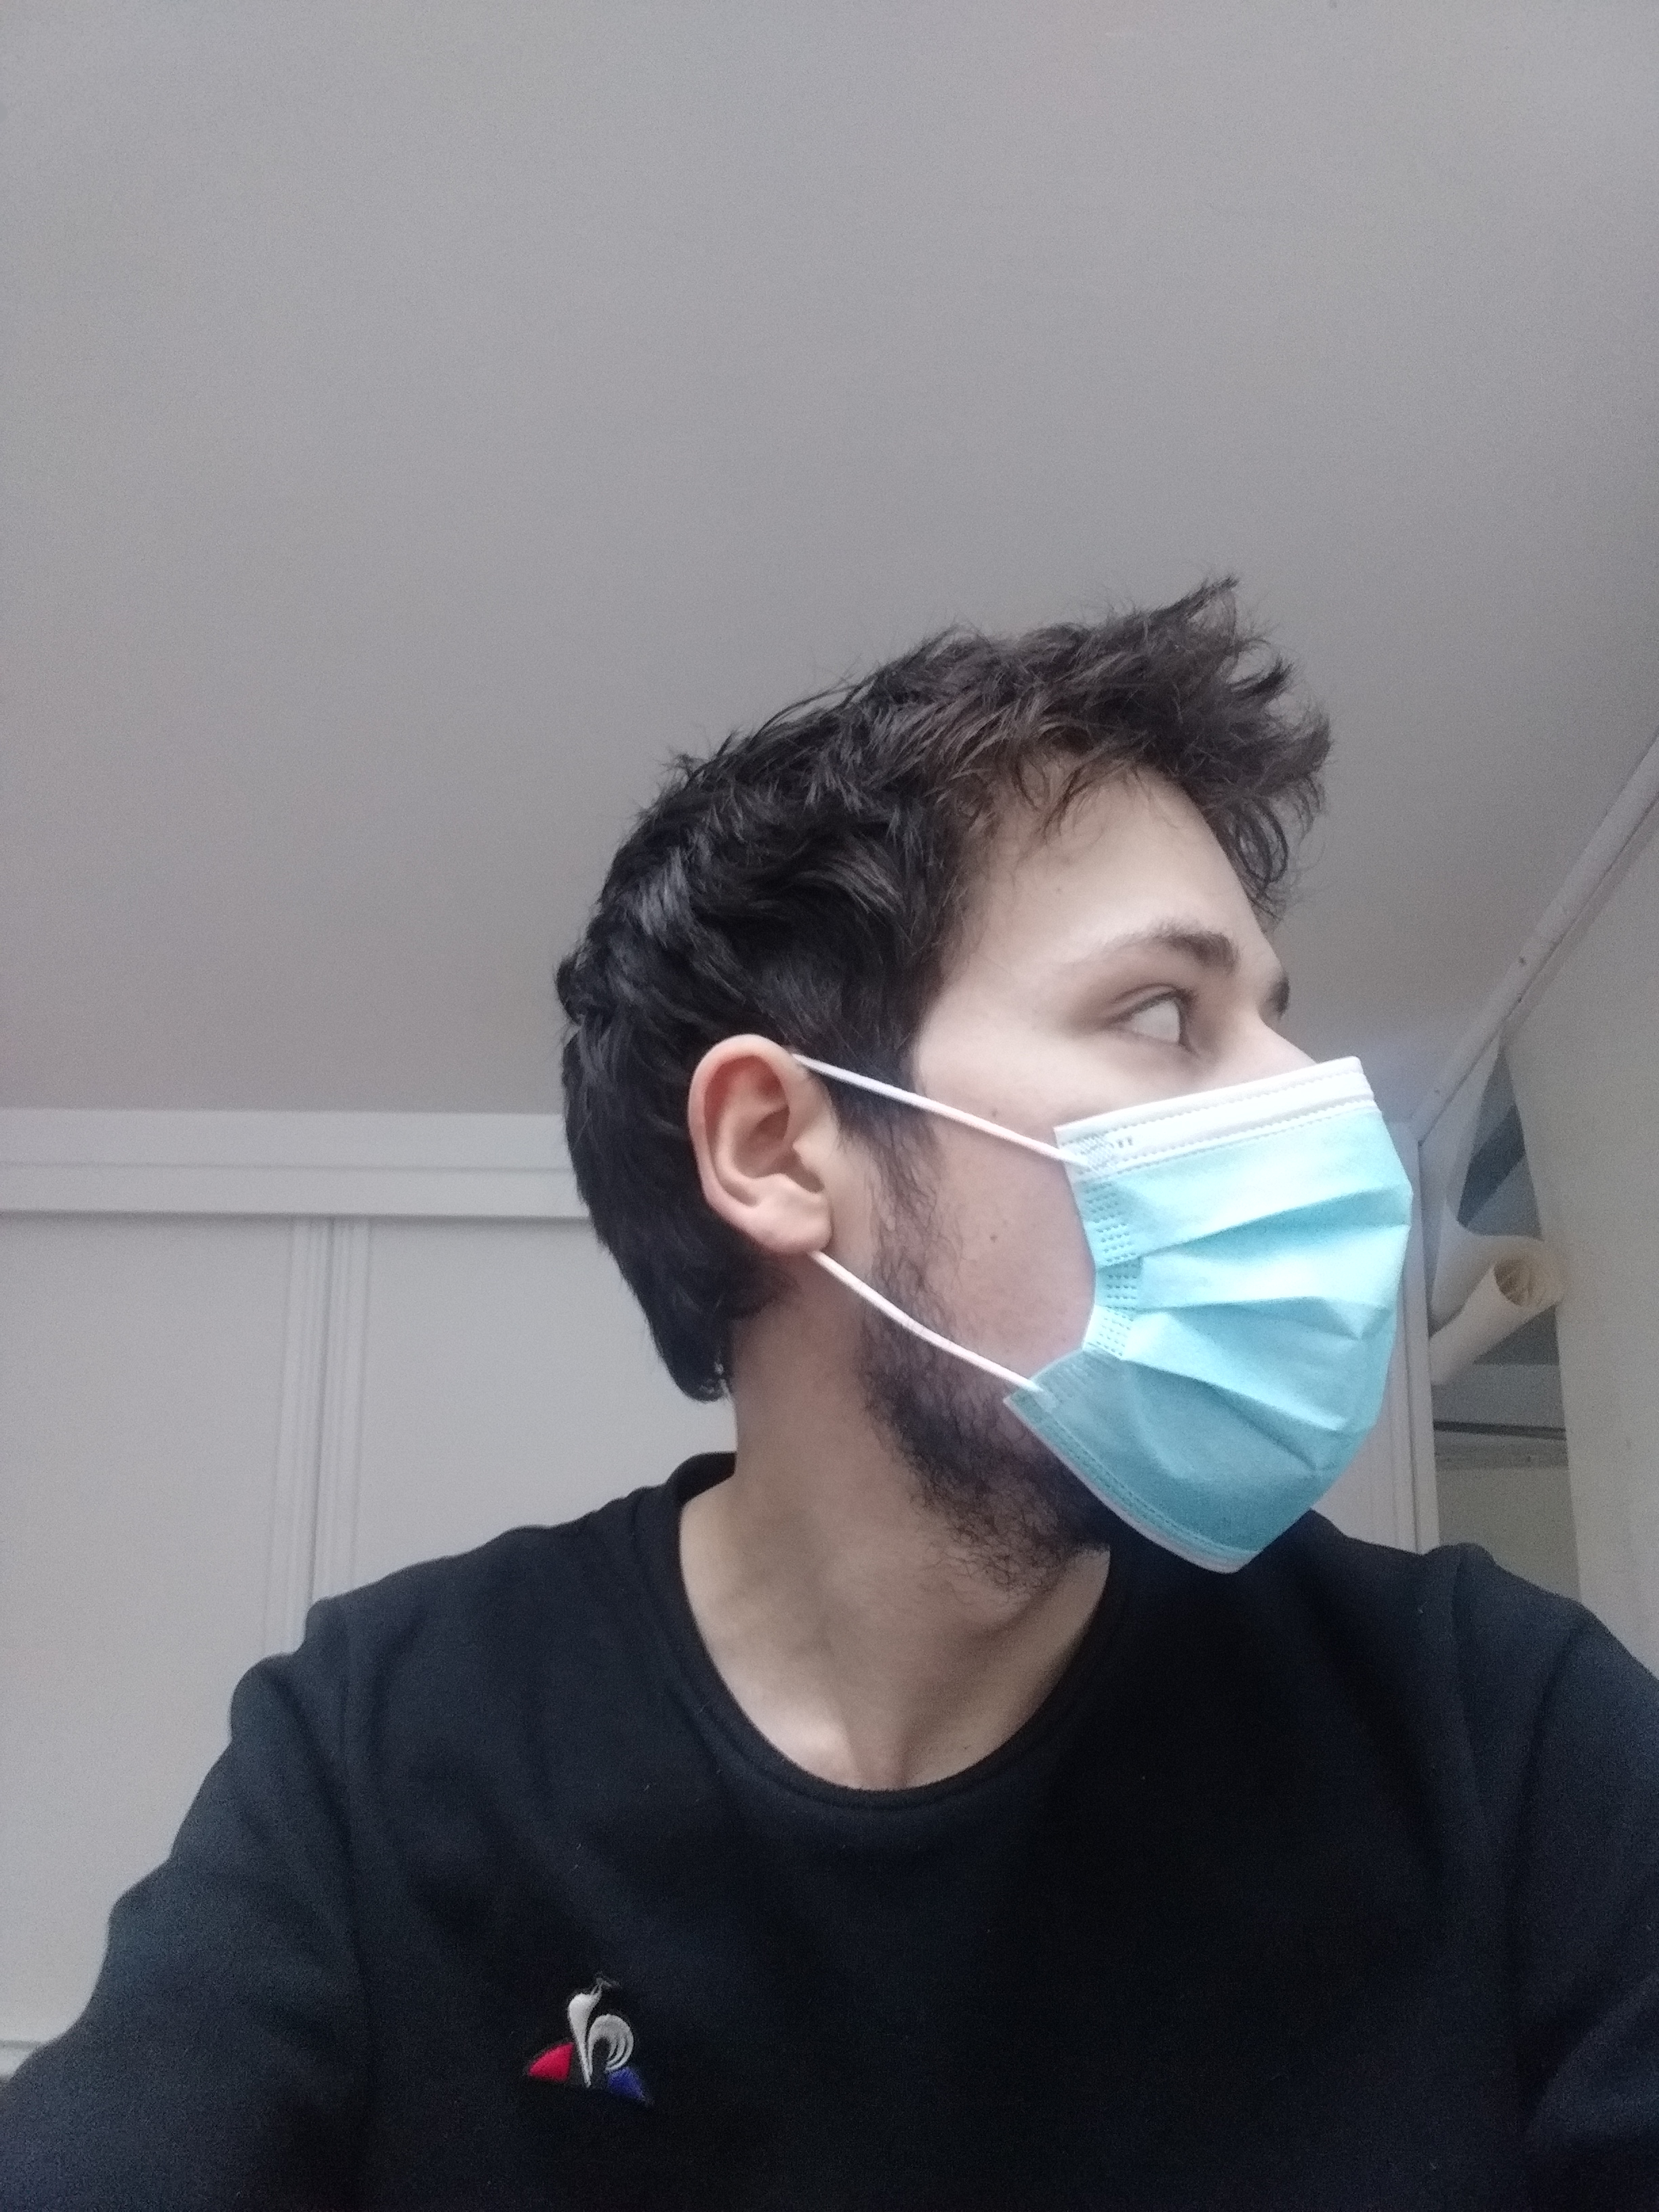
\includegraphics[width=0.2\textwidth]{20220115_150910.jpg}

\includegraphics[width=0.25\textwidth]{pred_categories.png}
\caption{\label{fig:Input}Deux exemples d'appels de la méthode predict avec deux photos. Pour la première, on demande des probabilités, et pour la seconde une catégorie. Le modèle d'extraction est d'abord appelé pour prédire un cadre pour le visage contenu dans la photo, puis le classificateur est appelé sur ce visage recadré.\\}
\end{figure}



\section{Conclusion}
Nos résultats montrent que nous avons répondu à la consigne avec succès. Notre modèle de classification a de très bonnes performances sur notre dataset. Notre modèle servant à extraire les visages pourrait largement être amélioré, mais il nous convient parfaitement dans le contexte de ce projet.\\
Pour obtenir de meilleurs résultats, nous pourrions commencer par rassembler plus de photos sous des angles encore plus variés, et avec des types de masque plus divers. Les résultats actuels sont très encourageants pour un dataset aussi restreint que le notre.\\ Dans un second temps, notre modèle d'extraction de visage nécessiterait plus d'expérimentations afin de diminuer son overfitting. Avec un dataset contenant plus de photos de groupe, nous pourrions aussi essayer de l'entraîner à extraire un nombre variable de visages depuis une seule photo.\\\\




\end{document}
